Molecular modeling seeks to gain new insights into the real world behavior of molecules by mimicing these molecules, usually using computer simulations.
Although quantum mechanics calculations are often viewed as the gold standard with respect to intramolecular energy calculations; 
having been used to parmeterize a majority of the most popular molecular mechanics force fields currently in use, including:
\begin{enumerate}
\item AMBER \cite{weiner1984new},
\item OPLS-AA \cite{kaminski1994free},
\item and CHARMM \cite{mackerell2002charmm}.
\end{enumerate}
Desipte the accuracy of quantum mechnics, its application to large systems such as proteins is currently limited due to the amount of time necessary to perform quantum mechanics calculations on a large number of atoms.
The earliest molecular mechanics force fields either modeled groups of atoms as a unit, hydrogens being grouped with their bound heavy atom \cite{jorgensen1988opls}, or even each residue as a unit \cite{lee1999energy}, both to reduce the number of parameters in the model and to increase the speed of computations.

\begin{figure}[H]
\begin{center}
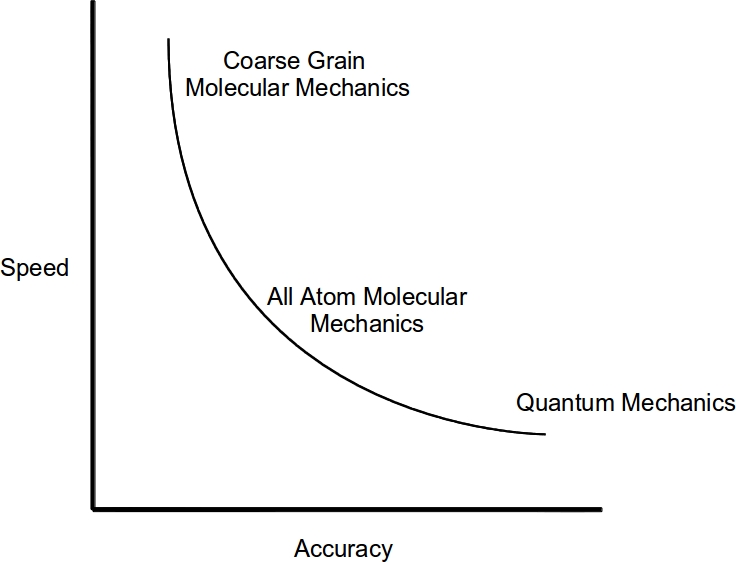
\includegraphics[width=0.7\textwidth]{figures/conservation_of_annoyance.png}
\caption{To an extent it is always possible to either increase accuracy or decrease running time, or the cost of an experiment.
New scientific methods should allow one to increase accuracy while not spending additional time.}
\label{figure:pdb_growth}
\end{center}
\end{figure}

\begin{equation}
E \left(r^N \right ) = E_\mathrm{bonds} + E_\mathrm{angles} + E_\mathrm{dihedrals} + E_\mathrm{nonbonded}
\label{equation:opls}
\end{equation}

\begin{equation}
E_\mathrm{bonds} = \sum_\mathrm{bonds} K_r (r-r_0)^2
\end{equation}

\begin{equation}
E_\mathrm{angles} = \sum_\mathrm{angles} k_\theta (\theta-\theta_0)^2
\end{equation}

\begin{equation}
E_\mathrm{dihedrals} = \sum_{i=1\dots4} {\frac {V_i} {2} \left [ 1 + \cos \left ( i * (\phi-\phi_0) \right ) \right ] }
\end{equation}

\begin{equation}
\begin{split}
E_\mathrm{nonbonded} = \sum_{i>j} f_{ij} 
                \left (
                        \frac {q_i q_j e^2}{r_{ij}}
                    + 4 \epsilon_{ij} 
                    \left  [  
                        \left ( \frac{\sigma_{ij}}{r_{ij}}\right )^{12}
                      - \left ( \frac{\sigma_{ij}}{r_{ij}}\right )^{6}
                    \right ]
                \right )
\\
f_{ij} = 
  \begin{dcases*}
   0    & if $i$ and $j$ are separated by 2 or fewer bonds\\
   0.5  & if $i$ and $j$ are separated by 3 bonds\\
   1.0  & otherwise
  \end{dcases*}
\end{split}
\end{equation}


Where $\sigma_{ij} = \sqrt{\sigma_{ii} \sigma_{jj}}$ and $\epsilon_{ij} = \sqrt{\epsilon_{ii}\epsilon_{jj}}$ \cite{jorgensen1996development}.
